% Thermocapillary (Marangoni) migration of a droplet -- introduction schematic.
% Companion to examples/2D_thermocapillary_migration (Samareh et al. 2014, Test Case 1).
%
% Compile:  pdflatex mechanism_schematic.tex   (or lualatex / tectonic)
%
% A drop in an imposed linear temperature field, oriented as the 2D case is: the gradient runs
% along +y (cold floor at the BOTTOM, hot ceiling at the TOP). Surface tension falls with T, so
% sigma varies CONTINUOUSLY around the interface -- drawn as a gradient: dark/heavy = high sigma
% on the cold (bottom) side, light/thin = low sigma on the hot (top) side. That tangential
% sigma-gradient is the Marangoni stress; it drives interfacial fluid hot -> cold (top -> bottom)
% and an internal recirculation, and by reaction the drop migrates UPWARD toward the hot ceiling (U).

\documentclass[border=4pt]{standalone}
\usepackage{amsmath}
\usepackage{tikz}
\usetikzlibrary{arrows.meta}

% restrained, print-friendly palette
\definecolor{coldc}{RGB}{46,86,149}
\definecolor{hotc}{RGB}{171,57,52}
\definecolor{marac}{RGB}{31,107,99}
\definecolor{flowc}{RGB}{125,125,125}
\definecolor{inkc}{RGB}{30,30,30}

\begin{document}
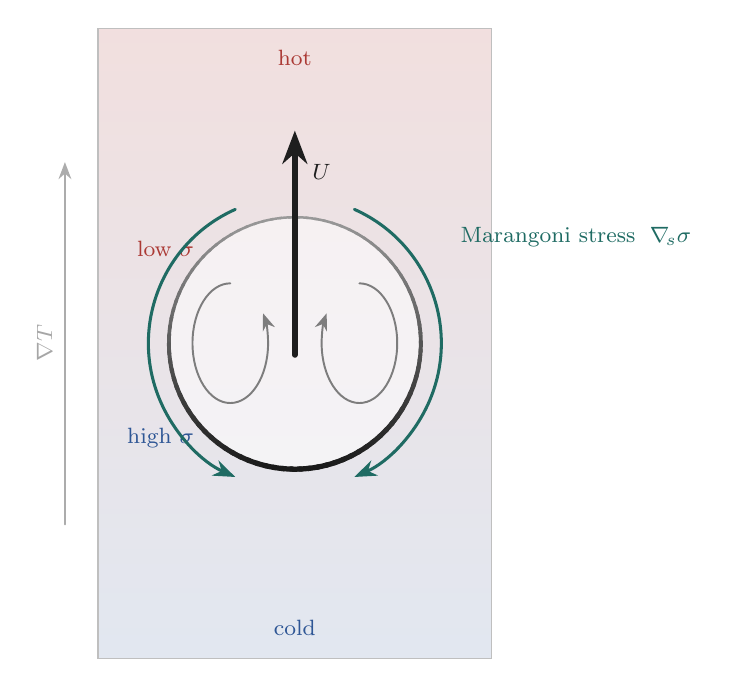
\begin{tikzpicture}[>=Stealth, font=\footnotesize, line cap=round]
  \def\R{1.6}

  % imposed temperature field (subtle) + thin domain frame: cold FLOOR (bottom) -> hot CEILING (top)
  \shade[bottom color=coldc!14, top color=hotc!16] (-2.5,-4) rectangle (2.5,4);
  \draw[gray!50, line width=0.4pt] (-2.5,-4) rectangle (2.5,4);
  \node[coldc] at (0,-3.62) {cold};
  \node[hotc]  at (0, 3.62) {hot};

  % temperature-gradient arrow: points UP (+y), along the left margin
  \draw[->, gray!65, line width=0.7pt] (-2.92,-2.3) -- (-2.92,2.3);
  \node[gray!70, rotate=90] at (-3.18,0) {$\nabla T$};

  % droplet interior (lightened so the interior arrows read cleanly)
  \fill[white, opacity=0.55] (0,0) circle (\R);

  % INTERFACE drawn as a gradient in sigma: each arc segment is shaded by its local
  % temperature (y = R sin a). cold/bottom -> high sigma (dark, heavy); hot/top -> low
  % sigma (light, thin). This is the surface-tension gradient that drives the flow.
  \foreach \a in {0,4,...,356}{
    \pgfmathsetmacro{\t}{(sin(\a)+1)/2}      % 0 at cold (bottom) pole, 1 at hot (top) pole
    \pgfmathsetmacro{\dk}{90-50*\t}          % line darkness  (high sigma -> dark)
    \pgfmathsetmacro{\lw}{1.9-1.0*\t}        % line weight    (high sigma -> heavy)
    \draw[black!\dk, line width=\lw pt] (\a:\R) arc[start angle=\a, end angle=\a+5, radius=\R];
  }
  \node[hotc,  anchor=east] at (-1.16, 1.20) {low $\sigma$};
  \node[coldc, anchor=east] at (-1.16,-1.20) {high $\sigma$};

  % Marangoni surface stress: tangential, hot -> cold (TOP -> BOTTOM) down the right and left sides
  \def\Mr{1.86}
  \draw[marac, line width=1.1pt, ->] (66:\Mr)  arc[start angle=66,  end angle=-66,  radius=\Mr];
  \draw[marac, line width=1.1pt, ->] (114:\Mr) arc[start angle=114, end angle=246,  radius=\Mr];
  \node[marac, anchor=west] at (1.98,1.35) {Marangoni stress $\;\nabla_{\!s}\sigma$};

  % internal recirculation (subtle): two vortices -- surface fluid down the sides, return up the middle
  \draw[flowc, line width=0.7pt, ->] (-0.82,0.76) arc[start angle=90, end angle=390,  x radius=0.48, y radius=0.76];
  \draw[flowc, line width=0.7pt, ->] ( 0.82,0.76) arc[start angle=90, end angle=-210, x radius=0.48, y radius=0.76];

  % migration of the drop toward the hot side = UPWARD
  \draw[inkc, line width=2.0pt, ->] (0,-0.15) -- (0,2.7);
  \node[inkc] at (0.34,2.18) {$U$};

\end{tikzpicture}
\end{document}
